\chapter{HASIL DAN PEMBAHASAN}

\section{Karakteristik Data}
Bagian ini memaparkan karakteristik data hasil praproses yang digunakan pada tahap pelatihan dan pengujian model, sebagaimana diuraikan pada Subbab 3.2.

\begin{table}[H]
\centering
\caption{Statistik ringkas himpunan data}
\label{tab:statistik-data}
\begin{tabular}{@{}lccc@{}}
\toprule
Himpunan & Jumlah Sampel & Jumlah Fitur & Proporsi (\%) \\
\midrule
Latih    & 0 & 0 & 70 \\
Validasi & 0 & 0 & 15 \\
Uji      & 0 & 0 & 15 \\
\bottomrule
\end{tabular}
\end{table}

\section{Hasil Pelatihan Model}
Gambar~\ref{fig:kurva-pelatihan} memperlihatkan kurva \textit{loss} pelatihan dan validasi terhadap jumlah iterasi (\textit{epoch}). Kurva ini digunakan untuk memantau kekonvergenan model serta mendeteksi indikasi \textit{overfitting}.

\begin{figure}[H]
\centering
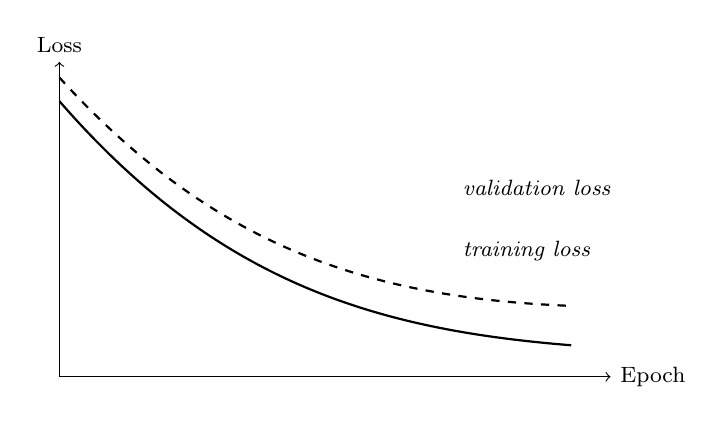
\begin{tikzpicture}
  \draw[->] (0,0) -- (7,0) node[right] {\footnotesize Epoch};
  \draw[->] (0,0) -- (0,4) node[above] {\footnotesize Loss};
  \draw[thick] (0,3.5) .. controls (2,1.2) and (4,0.6) .. (6.5,0.4);
  \draw[thick,dashed] (0,3.8) .. controls (2,1.6) and (4,1.0) .. (6.5,0.9);
  \node[anchor=west] at (5,1.6) {\footnotesize \textit{training loss}};
  \node[anchor=west] at (5,2.4) {\footnotesize \textit{validation loss}};
\end{tikzpicture}
\caption{Kurva \textit{loss} pelatihan dan validasi (ilustrasi)}
\label{fig:kurva-pelatihan}
\end{figure}

\section{Perbandingan Kinerja dengan Metode Pembanding}
Tabel~\ref{tab:hasil-perbandingan} menyajikan perbandingan kinerja pendekatan yang diusulkan dengan beberapa metode \textit{baseline} yang telah disebutkan pada Bab 2 \citep{russell2020,shukran2011}.

\begin{table}[H]
\centering
\caption{Perbandingan kinerja model}
\label{tab:hasil-perbandingan}
\begin{tabular}{@{}lccc@{}}
\toprule
Metode & Akurasi & F1-score & Waktu Komputasi (s) \\
\midrule
\textit{Baseline} 1 & 0.00 & 0.00 & 0.00 \\
\textit{Baseline} 2 & 0.00 & 0.00 & 0.00 \\
Metode yang Diusulkan & \textbf{0.00} & \textbf{0.00} & 0.00 \\
\bottomrule
\end{tabular}
\end{table}

\section{Pembahasan}
Hasil pada Tabel~\ref{tab:hasil-perbandingan} menunjukkan bahwa metode yang diusulkan memberikan kinerja \textit{[lebih baik/setara/dst.]} dibandingkan metode pembanding. Diskusikan di sini keterkaitan hasil dengan rumusan masalah pada Subbab 1.2 dan tinjauan pustaka pada Bab 2, termasuk kemungkinan penjelasan atas hasil yang diperoleh serta keterbatasannya.
